\documentclass{standalone}

\usepackage{amssymb}
\usepackage{amsmath}
\usepackage{tikz}
\usetikzlibrary{positioning}
\usetikzlibrary{arrows}

\newcommand{\R}{\mathbb{R}}
\newcommand{\D}{\mathrm{D}}

\begin{document}

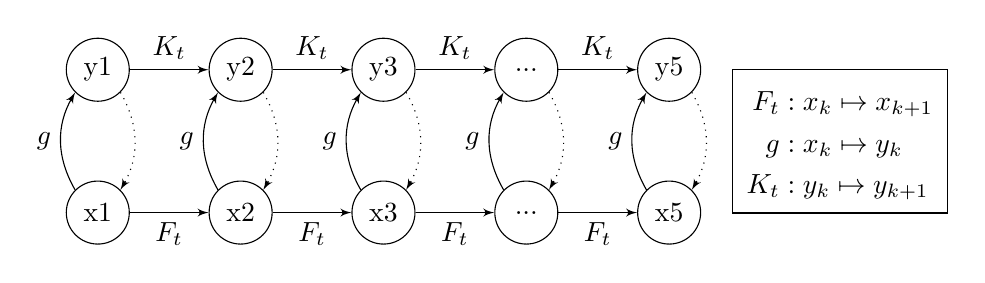
\begin{tikzpicture}[
roundnode/.style={circle, draw, minimum size=8mm},
vertex/.style={circle,draw,minimum size=1.5em},
edge/.style={->,> = latex'},
myblock/.style={draw}
]
%Nodes
\node[roundnode]        (t1)                            {y1};
\node[roundnode]        (t2)       [right=of t1]        {y2};
\node[roundnode]        (t3)       [right=of t2]        {y3};
\node[roundnode]        (t4)       [right=of t3]        {...};
\node[roundnode]        (t5)       [right=of t4]        {y5};

\node[roundnode]        (b1)       [below=of t1]       {x1};
\node[roundnode]        (b2)       [right=of b1]       {x2};
\node[roundnode]        (b3)       [right=of b2]       {x3};
\node[roundnode]        (b4)       [right=of b3]       {...};
\node[roundnode]        (b5)       [right=of b4]       {x5};


%Lines
\draw[edge] (t1.east) -- (t2.west) node[midway, above] {$K_t$};
\draw[edge] (t2.east) -- (t3.west) node[midway, above] {$K_t$};
\draw[edge] (t3.east) -- (t4.west) node[midway, above] {$K_t$};
\draw[edge] (t4.east) -- (t5.west) node[midway, above] {$K_t$};

\draw[edge] (b1.east) -- (b2.west) node[midway, below] {$F_t$};
\draw[edge] (b2.east) -- (b3.west) node[midway, below] {$F_t$};
\draw[edge] (b3.east) -- (b4.west) node[midway, below] {$F_t$};
\draw[edge] (b4.east) -- (b5.west) node[midway, below] {$F_t$};

\draw[edge,dotted] (t1.south east) to[bend left] (b1.north east);
\draw[edge] (b1.north west) to[bend left] node[midway, left] {$g$} (t1.south west) ;

\draw[edge, dotted] (t2.south east) to[bend left] (b2.north east);
\draw[edge] (b2.north west) to[bend left] node[midway, left] {$g$} (t2.south west);

\draw[edge, dotted] (t3.south east) to[bend left] (b3.north east);
\draw[edge] (b3.north west) to[bend left] node[midway, left] {$g$} (t3.south west);

\draw[edge, dotted] (t4.south east) to[bend left] (b4.north east);
\draw[edge] (b4.north west) to[bend left] node[midway, left] {$g$} (t4.south west);

\draw[edge, dotted] (t5.south east) to[bend left] node[name=rightmostedge]{} (b5.north east);
\draw[edge] (b5.north west) to[bend left] node[midway, left] {$g$} (t5.south west);

% text block on the right
% https://tex.stackexchange.com/questions/1342/aligned-equations-inside-of-tikz-node
 \node [rectangle, draw, right=0.2cm, text width=2.5cm, text height=0.7cm] (text) at (rightmostedge.east) {
        \begin{minipage}{\textwidth}
            \begin{align*}
                F_t&: x_k \mapsto x_{k+1} \\ 
                g&: x_k \mapsto y_k \\
                K_t&: y_k \mapsto y_{k+1}
            \end{align*}
        \end{minipage}
    };
 % Need this invisible node to leave white space at the right of the diagram...
 % Couldn't find a better way to do this.
 \node [rectangle, draw=none] (inv) at (text.east) {};
    
\end{tikzpicture}

\end{document}